\subsection{Glyph: \glyph{Equivalence arc} }\label{sec:equivalenceArc}

An \glyph{equivalence arc} is used to link a \glyph{tag} (\sect{tag}) or a \glyph{submap terminal} (\sect{submapTerminal}) to the \glyph{EPN} (\sect{EPNs}) or \glyph{compartment} (\sect{compartment}) it refers to.

\begin{glyphDescription}

\glyphSboTerm
Not applicable.

\glyphOrigin
One \glyph{EPN} (\sect{EPNs}) or \glyph{compartment} (\sect{compartment}).

\glyphTarget
One \glyph{tag} (\sect{tag}) or \glyph{submap terminal} (\sect{submapTerminal}).

\glyphSymbol No particular symbol is used to represent an \glyph{equivalence arc}, as shown in \fig{equivalenceArc}.
 \end{glyphDescription}

\begin{figure}[H]
  \centering
  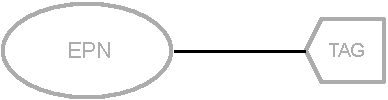
\includegraphics[scale = 0.8]{images/build/equivalence_arc.pdf}
  \caption{The \PD glyph for \glyph{Equivalence arc}.}
  \label{fig:equivalenceArc}
\end{figure}
